\documentclass[tikz]{standalone}

\usetikzlibrary{decorations.pathreplacing}

\usepackage{amssymb,stmaryrd}

\begin{document}
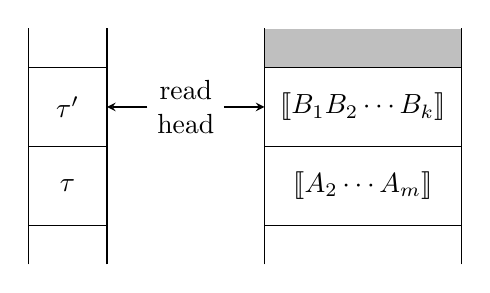
\begin{tikzpicture}[>=stealth,every text node part/.style={align=center}]

\draw [white,fill=lightgray] (3,2.5) rectangle +(2.5,-0.5);

%%%%%%%%%%%%%%%%%%%%%%%%%%%%%%%%%%%%%%

\draw [fill=none] (0,0) rectangle node {$\tau$}  +(1,1);
\draw [fill=none] (0,1) rectangle node {$\tau'$}  +(1,1);

%%%%%%%%%%%%%%%%%%%%%%%%%%%%%%%%%%%%%%

\draw [fill=none] (3,0) rectangle node {$\llbracket A_2 \cdots A_m \rrbracket$}  +(2.5,1);
\draw [fill=none] (3,1) rectangle node {$\llbracket B_1 B_2 \cdots B_k \rrbracket$}  +(2.5,1);

%%%%%%%%%%%%%%%%%%%%%%%%%%%%%%%%%%%%%%

\draw (0,-0.5) to +(0,3);
\draw (1,-0.5) to +(0,3);
\draw (3,-0.5) to +(0,3);
\draw (5.5,-0.5) to +(0,3);

\node(rh) at (2,1.5) {read\\head};
\draw[->] (rh) -- +(-1,0);
\draw[->] (rh) -- +(1,0);

\end{tikzpicture}
\end{document}
